\section*{Введение}
\addcontentsline{toc}{section}{Введение}

В процессе развития цифровых микросхем возникло противоречие между возможной
степенью интеграции и номенклатурой выпускаемых микросхем. Экономически
оправдано было выпускать микросхемы средней интеграции. Более сложные схемы
создавались из таких узлов, как регистры, счетчики, сумматоры. Разместить более
сложную схему на полупроводниковом кристалле было оправдано либо очень большой
серийностью аппаратуры, либо ценой аппаратуры (военная, авиационная или
космическая).

Для решения возникшей потребности в миниатюризации аппаратуры разработчикам
представили возможность изменять внутреннюю структуру микросхемы
(программировать).

История развития программируемых логических интегральных схем (ПЛИС) начинается
с появления программируемых постоянных запоминающих устройств. Первое время
программируемые ПЗУ использовались для хранения данных. Вскоре их стали
применять для реализации цифровых комбинаторных устройств с произвольной
таблицей истинности.  

\vspace*{2em} % ----------------------------------------------------------------

\section{Что такое ПЛИС. Области его применения}

ПЛИС (программируемые логические интегральные схемы) -- это большие
интегральные микросхемы матричного типа, позволяющие программным способом
реализовать логические функции большой сложности. Физическим ограничением
быстродействия присущей всем традиционным архитектурам процессоров является
последовательное выполнение команд. Всевозможные ухищрения вроде
суперскалярности, мультиконвейерности, многоядерности не сильно скрашивают эту
картину. Архитектура ПЛИС имеют потенциально большее быстродействие по
сравнению с микроконтроллерами и DSP процессорами. Это объясняется возможностью
аппаратного распараллеливания вычислений.

Основные области применения ПЛИС:
\begin{itemize}
    \item высокоскоростная обработка данных;
    \item алгоритмы ЦОС, особенно где требуется обработка данных в реальном
    времени;
    \item задачи обработки информации, требующие большого количества
    пользовательских выводов;
    \item промежуточный этап проектирования СБИС;
    \item узкоспециальные алгоритмы, построенные на жестких временных
    диаграммах;
    \item проекты, где требуется большое число портов ввода-вывода.
\end{itemize}

\vspace*{2em} %  ----------------------------------------------------------------

\section{Простейшие ПЛИС - программируемые логические матрицы (ПЛМ)}

Программируемые логические матрицы -- наиболее традиционный тип ПЛИС, имеющий
программируемые матрицы ``И'' и ``ИЛИ''. 
Примерами таких ПЛИС могут служить отечественные схемы K556PT1, PT2, PT21.

Построение ПЛМ основано на том, что любая комбинационная функция может быть
представлена в виде логической суммы (операция ИЛИ) логических произведений
(операций И). Тогда схема реализующая комбинационную функцию может быть
представлена в виде, показанном на рисунке \ref{pic_2}.

\begin{figure}[h!]
    \centering
    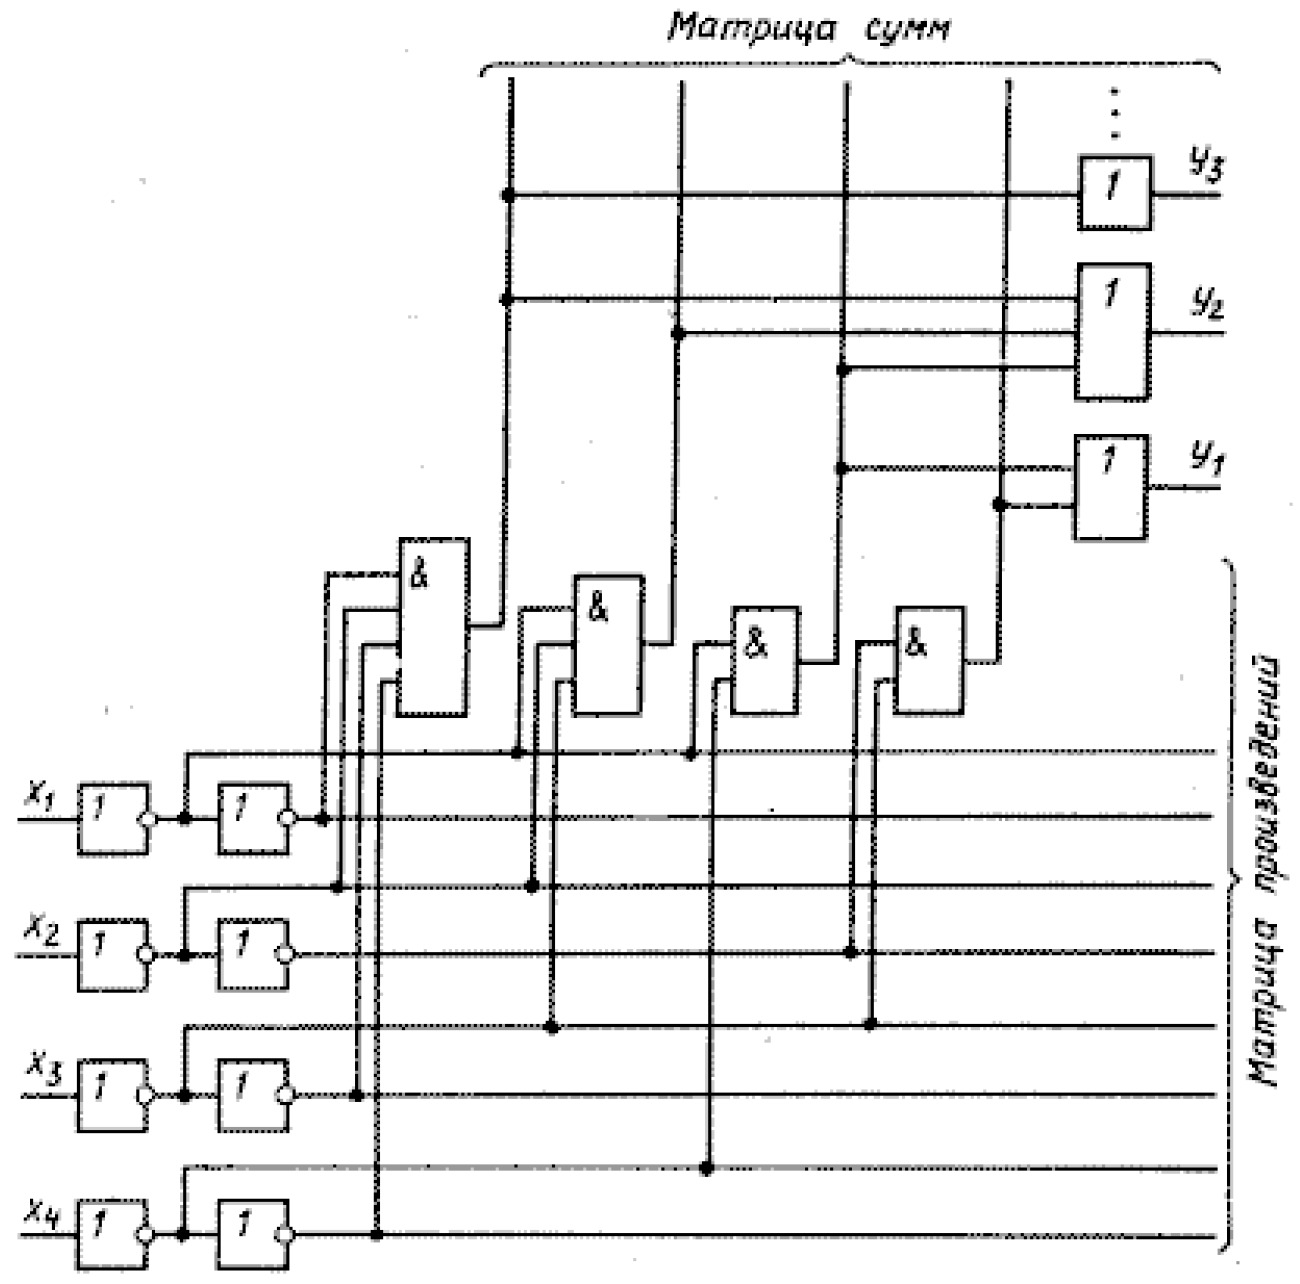
\includegraphics[width=.5\textwidth]{pld}
    \caption{Представление комбинационной функции}
    \label{pic_2}
\end{figure}

Недостаток такой архитектуры -- слабое использование ресурсов программируемой
матрицы ``ИЛИ'', поэтому дальнейшее развитие получили микросхемы, построенные
по архитектуре программируемой матричной логики (PAL - \emph{Programmable Array
Logic}) - это ПЛИС, имеющие программируемую матрицу ``И'' и фиксированную
матрицу ``ИЛИ''. К этому классу относятся большинство современных ПЛИС
небольшой степени интеграции. Разновидностью этого класса являются ПЛИС,
имеющие только одну (программируемую) матрицу ``И'', например, схема 85C508
фирмы INTEL. Следующий традиционный тип ПЛИС~-- программируемая макрологика.
Они содержат единственную программируемую матрицу ``И-НЕ'' или ``ИЛИ-НЕ'', но
за счёт многочисленных инверсных обратных связей способны формировать сложные
логические функции. 

Вышеперечисленные архитектуры ПЛИС содержат небольшое число ячеек, к настоящему
времени устарели и применяются для реализации относительно простых
устройств, для которых не существует готовых ИС средней степени интеграции.
Для реализации алгоритмов ЦОС они непригодны.

\vspace*{2em}
% ------------------------------------------------------------------

\section*{Заключение}
\addcontentsline{toc}{section}{Заключение}

Стремительные преобразования такие, как количественные (увеличение плотности
ячеек на кристалле), множество качественных (разработка новых архитектур) и
принципиально новых подходов прошедшие в производстве ПЛИС за
сравнительно короткое время дают повод полагать, что, с одной стороны, вновь
выпускаемые ИС получат более высокие технические показатели, с другой --
предлагаемые решения более низкой ценовой категории будут занимать все больше
места в приложениях, где до сегодняшнего дня использовались традиционные
методы: ИС стандартной логики и БИС.

\vspace*{2em} % ----------------------------------------------------------------
\renewcommand{\bibname}{Список источников}

\begin{thebibliography}{9} \addcontentsline{toc}{section}{Список источников}
    \bibitem{1} \href{http://de.ifmo.ru/bk_netra/page.php?tutindex=25&index=43}
    {http://de.ifmo.ru/bk\_netra/page.php?tutindex=25\&index=43}
    \bibitem{2} \href{http://www.chipovod.ru/category/plis/}
    {http://www.chipovod.ru/category/plis/}
    \bibitem{3} \href{http://digteh.ru/digital/PLD/}
    {http://digteh.ru/digital/PLD/}
\end{thebibliography}